\section{Câbles}
\subsection{La bande passante}
La bande passante correspond à la plage de fréquences à une distance donnée.
\subsection{Mode série vs mode parallèle}
\begin{figure}[H]
  \centering
  \begin{minipage}{.45\textwidth}
    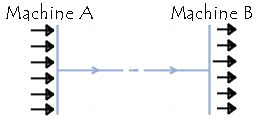
\includegraphics[width=\textwidth]{img/serie.jpg}
    \caption{Schéma d'une liaison série}
    \label{img:1}
  \end{minipage}
  ~
  \begin{minipage}{.45\textwidth}
    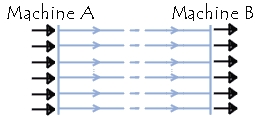
\includegraphics[width=\textwidth]{img/parallele.jpg}
    \caption{Schéma d'une liaison parallèle}
    \label{img:2}
  \end{minipage}
  \caption*{Comparaison entre la liaison série et la liaison parallèle}
\end{figure}
Comme nous pouvons le voir sur les schéma ci-dessus (\ref{img:1} et \ref{img:2}), le mode de liaison série va permettre d'économiser beaucoup de câbles et ainsi de faire des économies.\\
Le mode de liaison parallèle va être beaucoup plus cher à mettre en place, va demander plus de place et va être beaucoup plus susceptible aux interférences inter-câbles.
\subsection{Protection contre les interférences}
\begin{description}
 \item[Blindage (Shield)] Protège des l'intrusion de parasites de hautes fréquences dans le câble. Permet aussi de s'assurer que le signal du câble ne s'échappe pas à l'extérieur.
 \item[Écrantage (Folded)] Protège de l'intrusion de parasites de basses fréquences ($< 3000Hz$) dans le câble.
\end{description}
Le meilleur compromis, pour le moment, est d'avoir une câble S/FTP : le câble entier est blindé (S) puis chaque paire est écrantée (FTP\footnote{Folded Twisted Pair}).
\subsection{Distance maximum}
Entre deux EAR\footnote{Équipements Actifs de Réseau}, il ne faut pas dépasser une distance maximale de 100m.
\subsection{POE}
Le POE\footnote{Power Over Ethernet} permet d'alimenter certains équipements en utilisant un câble Ethernet.

\section{IP/Ethernet}
\subsection{MAC}
La MAC\footnote{Media Access Control} address a été normalisée par l'IEEE\footnote{Institute of Electrical and Electronics Engineers}.\\
Il existe deux notations utilisée pour les MAC address utilisée :
\begin{description}
 \item[IEEE] $01:23:45:67:89:AB$
 \item[IBM] $01-23-45-67-89-AB$
\end{description}
\subsection{Ethernet}
\begin{figure}[H]
  \centering
  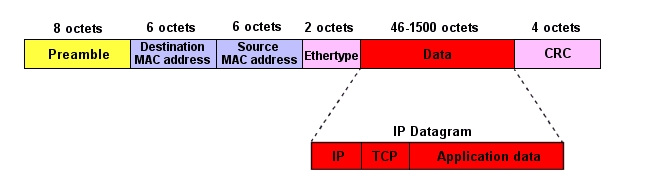
\includegraphics[width=.9\textwidth]{img/ethernetFrame.jpg}
  \label{img:3}
  \caption{Représentation des éléments d'une trame Ethernet}
\end{figure}
La longueur maximale d'une trame Ethernet est de $1518$ Bytes (octets).\\
La trame de broadcast Ethernet est notée de la manière suivante : $FF:FF:FF:FF:FF:FF$.\\
Au sein d'une trame Ethernet, nous allons pouvoir retrouver le type\footnote{Frame Type}. Ce dernier va permettre de définir quel type de données est contenue dans le payload. La carte pourra ainsi envoyer les données au bon protocole par la suite.

\section{Matériel}
\subsection{Switch}
Les switchs sont des équipements full-duplex. La communication peut circuler dans les deux sens à n'importe quel moment. Il n'y a ainsi pas de collisions possible.\\
La mémoire des switch est appelée CAM\footnote{Content Addressable Memory}. Cette CAM permet de réaliser des recherches rapide de contenance de mot dans la mémoire.

\section{Adresses IP}
\subsection{Réseaux privés}
Il existe trois plages de réseaux privées (qu'on ne retrouvera pas sur les réseau publiques) :
\begin{itemize}
 \item $192.168.0.0/16$
 \item $172.16.0.0/12$
 \item $10.0.0.0/8$
\end{itemize}
En cas de problème de connexion, il faut dans réaliser les étapes suivantes dans l'ordre pour déterminer la localisation du problème :
\begin{enumerate}
 \item PING du routeur
 \item PING du DNS
 \item PING du nom de domaine
\end{enumerate}
\subsection{Classes d'adresses}
\begin{description}
 \item[Classe A] Sur ce type de réseau, il est possible d'avoir $2^{3*8}-2=2^{24}-2=16777214$ terminaux. Le masque de sous-réseau est de $255.0.0.0$, soit un $/8$.\\Le premier octet d'une adresse IP de classe A commence toujours par le bit 0, il est donc compris entre 0 et 127, certaines valeurs étant réservées à des usages particuliers. Un exemple d'adresse IP de classe A est : $10.50.49.13$.
 \item[Classe B] Sur ce type de réseau, il est possible d'avoir $2^{2*8}-2=2^{16}-2=65534$ terminaux. Le masque de sous-réseau est de $255.255.0.0$, soit un $/16$.\\Le premier octet d'une adresse IP de classe B commence toujours par la séquence de bits 10, il est donc compris entre 128 et 191. Un exemple d'adresse IP de classe B est : $172.16.1.23$.
 \item[Classe C] Sur ce type de réseau, il est possible d'avoir $2^{8}-2=254$ terminaux. Le masque de sous-réseau est de $255.255.255.0$, soit un $/24$.\\Le premier octet d'une adresse IP de classe C commence toujours par la séquence de bits 110, il est donc compris entre 192 et 223. Un exemple d'adresse IP de classe C est : $192.168.1.34$.
 \item[Classe D] Les adresses de classe D sont utilisées pour les communications multicast. Le premier octet d'une adresse IP de classe D commence toujours par la séquence de bits 1110, il est donc compris entre 224 et 239. Un exemple d'adresse IP de classe D est : $224.0.0.1$.
 \item[Classe E] Les adresses de classe E sont réservées par IANA\footnote{Internet Assigned Numbers Authority} à un usage non déterminé. Les adresses de classe E commencent toujours par la séquence de bits 1111, ils débutent donc en 240.0.0.0 et se terminent en 255.255.255.255.
\end{description}

\subsection{Exemples}
\begin{itemize}
 \item L'adresse de broadcast du réseau $15.15/16$ est $16.16.255.255$.
 \item L'adresse IP du réseau de $172.16.0.1/24$ est $172.16.0.0/24$.
 \item Un réseau de classe C contient 256 adresses ($2^8$) mais ne peut contenir un maximum de 254 équipements réseaux ($2^{8}-2$).
\end{itemize}
